\documentclass{standalone}
\usepackage{tikz}
\usepackage{float}
\usepackage{amsmath}
\usepackage{lmodern}
\usepackage{amssymb}
\usetikzlibrary{calc}
\usetikzlibrary{hobby}
\usepackage{nicefrac}
\usetikzlibrary{decorations.markings}
\usetikzlibrary{patterns, patterns.meta}
\usetikzlibrary{shapes}
\usetikzlibrary{shapes.misc}
\usepackage{pgfplots}
\pgfplotsset{compat=1.18}
\begin{document}
\centering

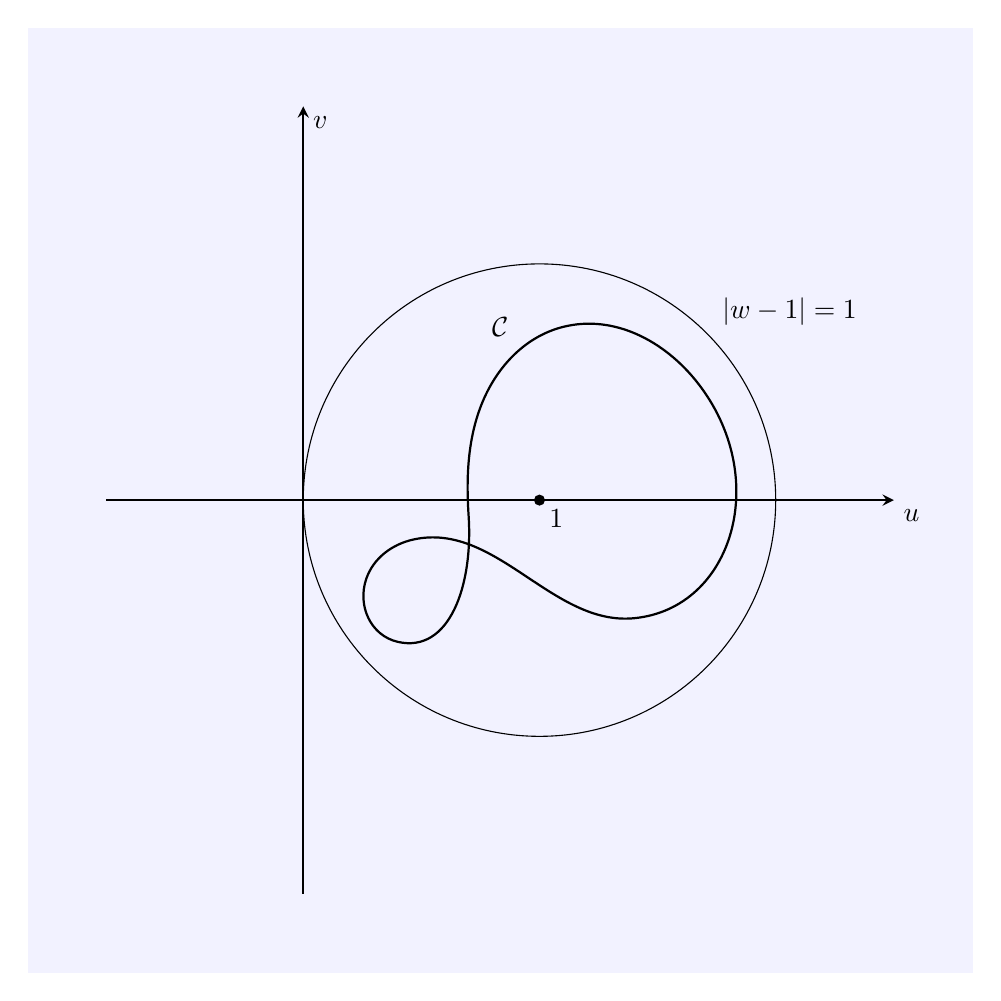
\begin{tikzpicture}
    \tikzset{arrowstyle/.style={->, >=stealth}}

    \colorlet{BlueBackground}{blue!5}
    % Background for entire canvas
    \fill[BlueBackground] (-6,-6) rectangle (6,6);
    % Assen
    \draw[thick, arrowstyle] ($(-5,0)$) -- ($(5,0)$);
    \draw[thick, arrowstyle] ($(-2.5,-5)$) -- ($(-2.5,5)$);
    \coordinate (x) at (5,0);
    \draw (x) node[below right] {$u$};
    \coordinate (y) at (-2.5,5);
    \draw (y) node[below right] {$v$};
    % 1 
    \coordinate (1) at (0.5,0);
    \fill (1) circle (2pt);
    \draw (1) node[below right] {$1$};
    % Cirkel
    \draw(3.5,0) arc[start angle=0, end angle=-360, radius=3];
    \coordinate (W) at (2.7,2.7);
    \draw (W) node[below right] {$|w-1|=1$};
    % draw contour
    \path [draw=black,thick]
    (2.5,1.5) to[closed, curve through =
    { (0.8,2.2) (-0.2,1.3) (-0.4,-0.2) (-1.3,-1.8) (-1.7,-1) (-1.1,-0.5) }] (1.7,-1.5);
    \node at (0,2.2) {\textcolor{black}{$\mathcal{C}$}};

    
\end{tikzpicture}

\end{document}